\section{The Heat Equation}

\vskip14pt

\noindent
We begin the study of partial differential equations with the problem of heat flow in a uniform bar
of length $L$, situated on the $x$ axis with one end at the origin and the other at $x=L$
(Figure~\ref{figure:12.1.1}).

%\begin{figure}[tbp]
%  \centering\color{blue}
%  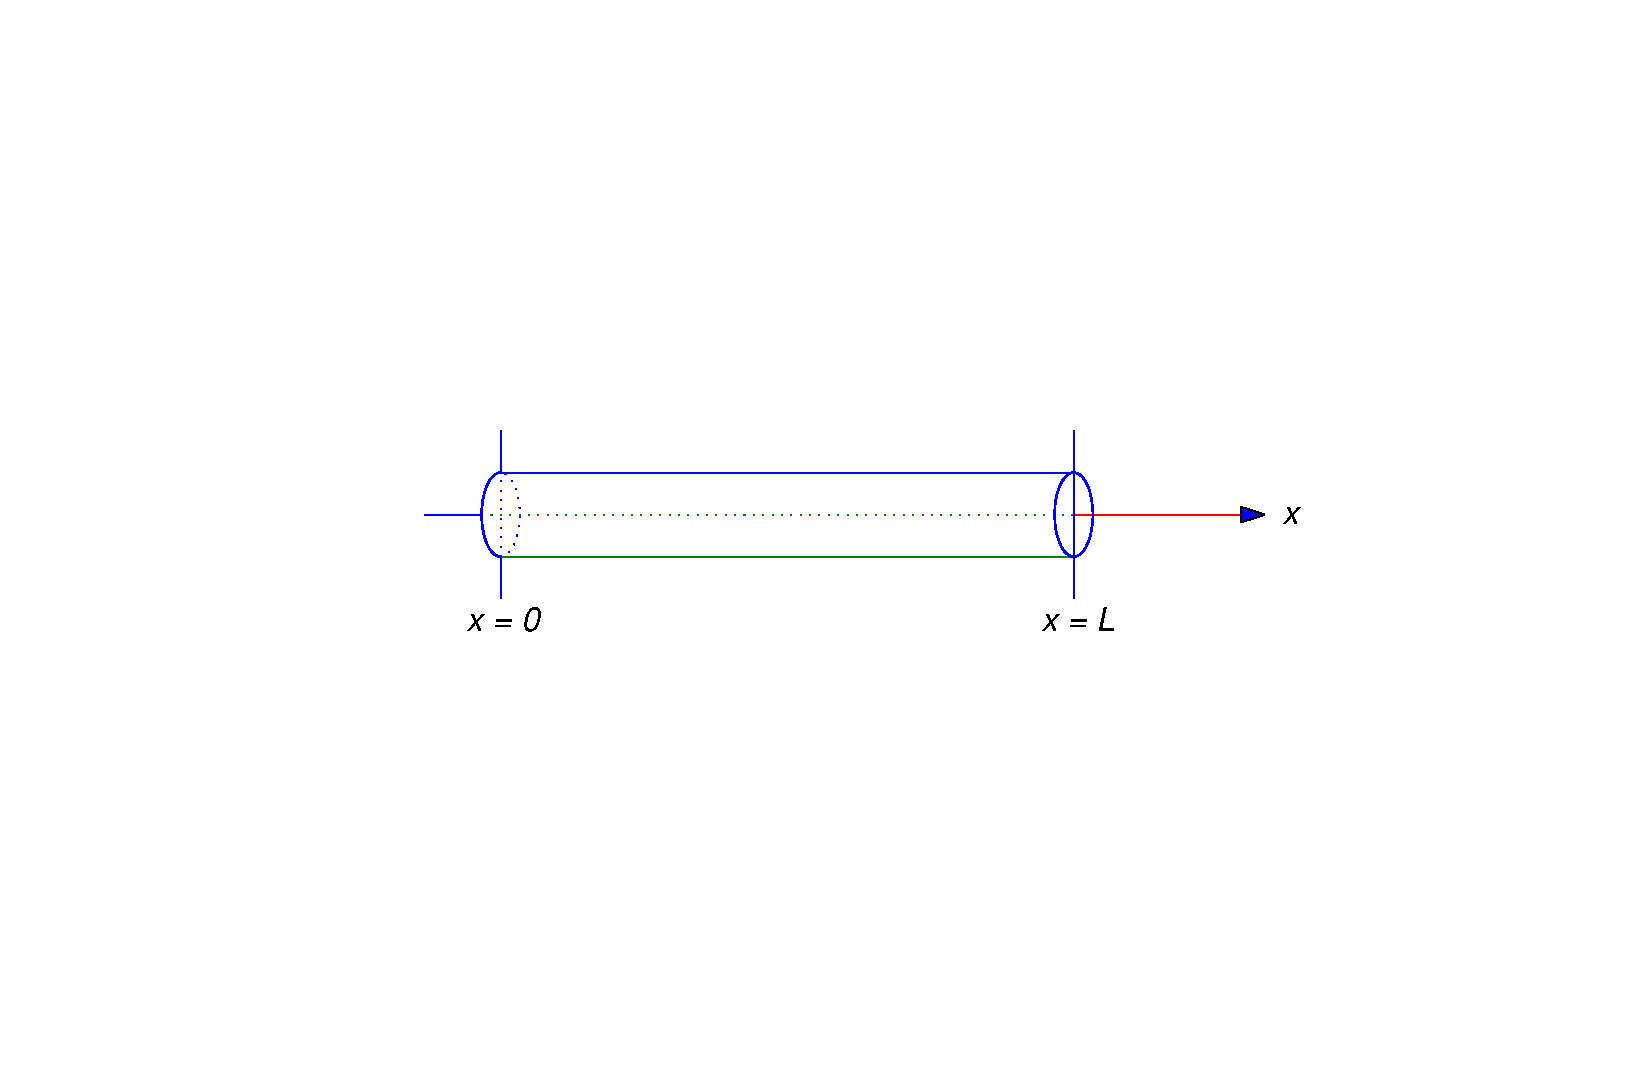
\includegraphics[bb=-78 148 689 643,width=5.67in,height=3.66in,keepaspectratio]{fig120101}
%\caption{A uniform bar of length $L$}
%  \label{figure:12.1.1}
%\end{figure}

We assume that the bar is perfectly insulated except possibly at its endpoints, and that the
temperature is constant on each cross section and therefore depends only on $x$ and $t$. We also
assume that the thermal properties of the bar are independent of $x$ and $t$. In this case, it can
be shown that the temperature $u=u(x,t)$ at time~$t$ at a point $x$ units from the origin satisfies
the partial differential equation
\[
  u_{t}=a^{2}u_{xx},\quad0<x<L,\quad t>0,
\]
where $a$ is a positive constant determined by the thermal properties. This is the {\color{blue}\it
heat equation\/}.

\vspace*{-.2in}
\begin{figure}[H]
  \centering
  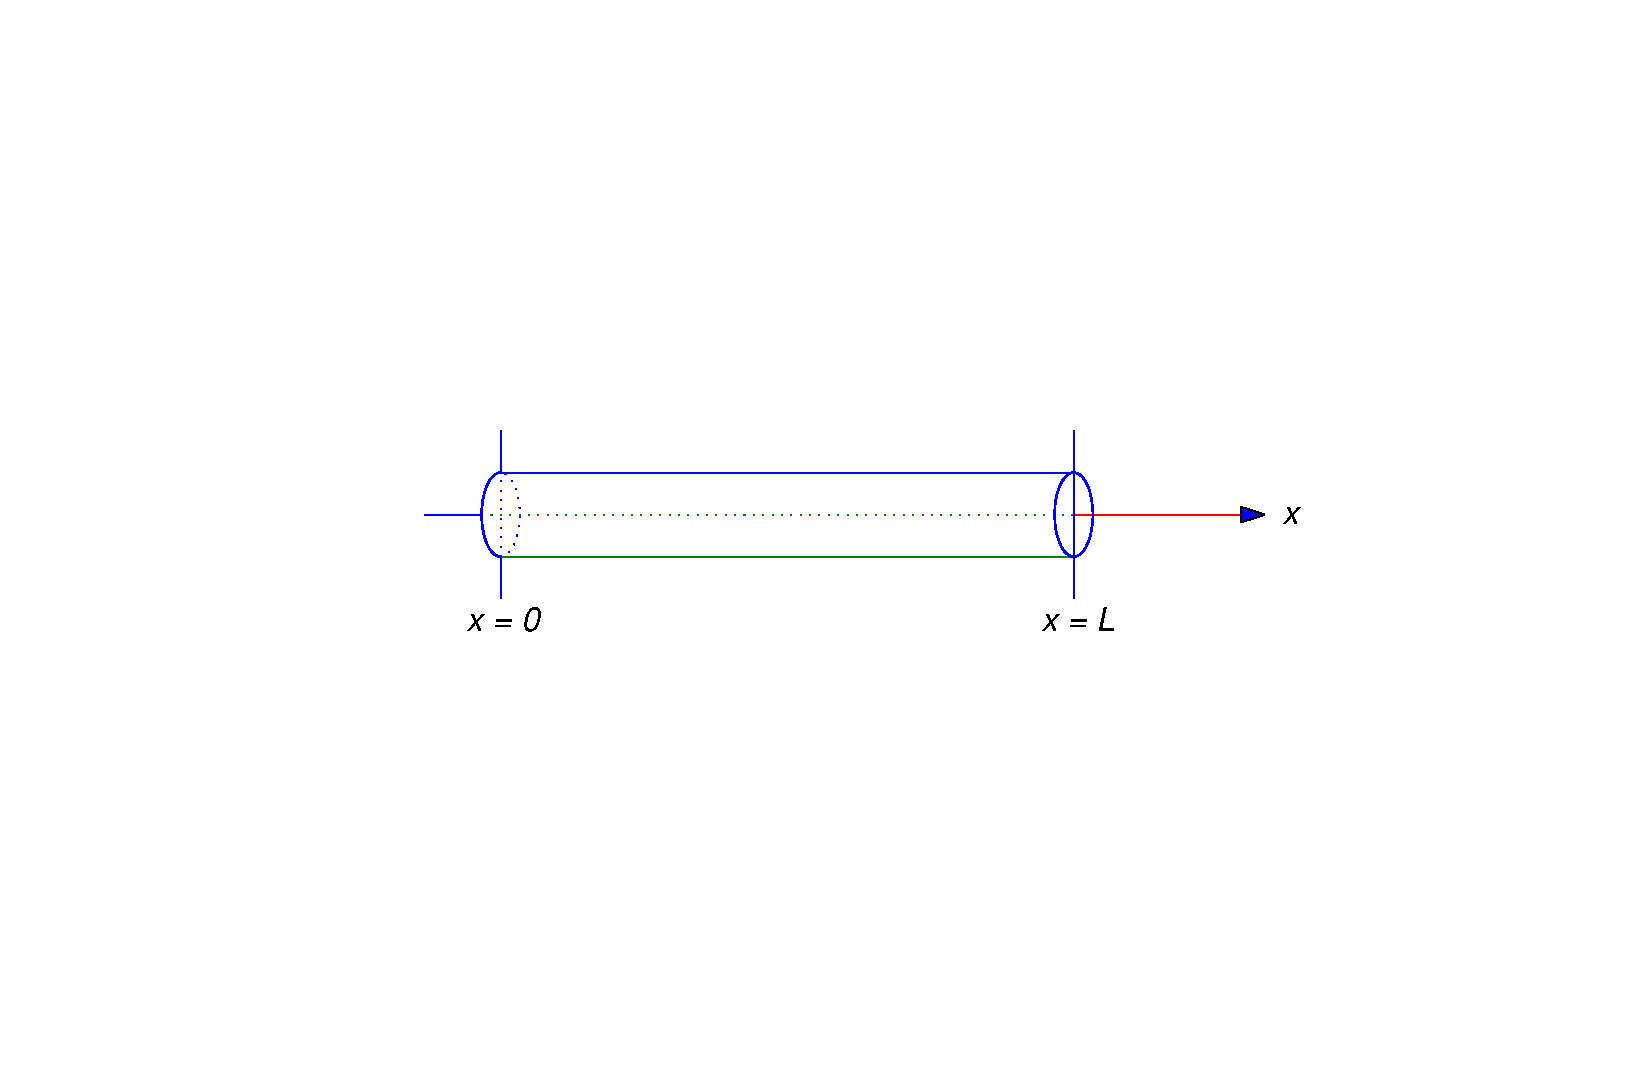
\includegraphics[bb=-78 148 689 643, width=5.67in, height=3.66in, keepaspectratio]{fig120101}
  \vspace*{-1in}
  \caption{A uniform bar of length $L$}
  \label{figure:12.1.1}
\end{figure}

To determine $u$, we must specify the temperature at every point in the bar when $t=0$, say
\[
  u(x,0)=f(x),\quad0\le x\le L.
\]
We call this the {\color{blue}\it initial\/} condition. We must also specify {\color{blue}\it
boundary conditions\/} that $u$ must satisfy at the ends of the bar for all $t>0$. We'll call this
problem an {\color{blue}\it initial-boundary value problem.\/}

We begin with the boundary conditions $u(0,t)=u(L,t)=0$, and write the initial-boundary value
problem as
\begin{equation}
  \label{eq:12.1.1}
  \begin{array}{c}
    u_{t}=a^{2}u_{xx},\quad0<x<L,\quad t>0, \\
    u(0,t)=0,\quad u(L,t)=0,\quad t>0,      \\
    u(x,0)=f(x),\quad0\le x\le L.
  \end{array}
\end{equation}
Our method of solving this problem is called {\color{blue}\it separation of variables\/} (not to be
confused with method of separation of variables used in Section~2.2 for solving ordinary
differential equations). We begin by looking for functions of the form
\[
  v(x,t)=X(x)T(t)
\]
that are not identically zero and satisfy
\[
  v_{t}=a^{2}v_{xx},\quad v(0,t)=0,\quad v(L,t)=0
\]
for all $(x,t)$. Since
\[
  v_{t}=XT'\mbox{\quad and \quad}v_{xx}=X''T,
\]
$v_{t}=a^{2}v_{xx}$ if and only if
\[
  XT'=a^{2}X''T,
\]
which we rewrite as
\[
  \frac{T'}{a^{2}T}=\frac{X''}{X}.
\]
Since the expression on the left is independent of $x$ while the one on the right is independent of
$t$, this equation can hold for all $(x,t)$ only if the two sides equal the same constant, which we
call a {\color{blue}\it separation constant\/}, and write it as $-\lambda$; thus,
\[
  \frac{X''}{X}=\frac{T'}{a^{2}T}=-\lambda.
\]
This is equivalent to
\[
  X''+\lambda X=0
\]
and
\begin{equation}
  \label{eq:12.1.2}T'=-a^{2}\lambda T.
\end{equation}
Since $v(0,t)=X(0)T(t)=0$ and $v(L,t)=X(L)T(t)=0$ and we don't want $T$ to be identically zero,
$X(0)=0$ and $X(L)=0$. Therefore $\lambda$ must be an eigenvalue of the boundary value problem
\begin{equation}
  \label{eq:12.1.3}X''+\lambda X=0,\quad X(0)=0,\quad X(L)=0,
\end{equation}
and $X$ must be a $\lambda$-eigenfunction. From Theorem~\ref{thmtype:11.1.2}, the eigenvalues of
\eqref{eq:12.1.3} are $\lambda_{n}=n^{2}\pi^{2}/L^{2}$, with associated eigenfunctions
\[
  X_{n}=\sin\frac{n\pi x}{L},\quad n=1,2,3,\dots.
\]
Substituting $\lambda=n^{2}\pi^{2}/L^{2}$ into \eqref{eq:12.1.2} yields
\[
  T'=-(n^{2}\pi^{2}a^{2}/L^{2})T,
\]
which has the solution
\[
  T_{n}=e^{-n^{2}\pi^{2}a^{2}t/L^{2}}.
\]
Now let
\[
  v_{n}(x,t)=X_{n}(x)T_{n}(t)=e^{-n^{2}\pi^{2}a^{2}t/L^{2}}\sin\frac{n\pi x}{L},\quad n=1,2,3,\dots
\]
Since
\[
  v_{n}(x,0)=\sin\frac{n\pi x}{L},
\]
$v_{n}$ satisfies \eqref{eq:12.1.1} with $f(x)=\sin n\pi x/L$. More generally, if
$\alpha_{1},\dots,\alpha_{m}$ are constants and
\[
  u_{m}(x,t)= \sum_{n=1}^{m}\alpha_{n}e^{-n^{2}\pi^{2}a^{2}t/L^{2}}\sin\frac{n\pi x}{L},
\]
then $u_{m}$ satisfies \eqref{eq:12.1.1} with
\[
  f(x)=\sum_{n=1}^{m}\alpha_{n}\sin\frac{n\pi x}{L}.
\]
This motivates the next definition.

\begin{definition}
  \color{blue}
  \label{thmtype:12.1.1}\rm The {\color{blue}\it formal solution\/} of the initial-boundary value
  problem
  \begin{equation}
    \label{eq:12.1.4}
    \begin{array}{c}
      u_{t}=a^{2}u_{xx},\quad0<x<L,\quad t>0, \\
      u(0,t)=0,\quad u(L,t)=0,\quad t>0,      \\
      u(x,0)=f(x),\quad0\le x\le L
    \end{array}
  \end{equation}
  is
  \begin{equation}
    \label{eq:12.1.5}u(x,t)=\sum_{n=1}^{\infty}\alpha_{n}e^{-n^{2}\pi^{2}a^{2}t/L^{2}}\sin\frac{n\pi x}{L},
  \end{equation}
  where
  \[
    S(x)=\sum_{n=1}^{\infty}\alpha_{n}\sin\frac{n\pi x}{L}
  \]
  is the Fourier sine series of $f$ on $[0,L]$; that is,
  \[
    \alpha_{n}=\frac{2}{L}\int_{0}^{L}f(x)\sin\frac{n\pi x}{L}\,dx.
  \]
\end{definition}

We use the term ``formal solution'' in this definition because it's not in general true that the
infinite series in \eqref{eq:12.1.5} actually satisfies all the requirements of the initial-boundary
value problem \eqref{eq:12.1.4} when it does, we say that it's an {\color{blue}\it actual
solution\/} of \eqref{eq:12.1.4}.

Because of the negative exponentials in \eqref{eq:12.1.5}, $u$ converges for all $(x,t)$ with $t>0$
(Exercise~\ref{exer:12.1.54}). Since each term in \eqref{eq:12.1.5} satisfies the heat equation and
the boundary conditions in \eqref{eq:12.1.4}, $u$ also has these properties if $u_{t}$ and $u_{xx}$
can be obtained by differentiating the series in \eqref{eq:12.1.5} term by term once with respect to
$t$ and twice with respect to $x$, for $t>0$. However, it's not always legitimate to differentiate
an infinite series term by term. The next theorem gives a useful sufficient condition for legitimacy
of term by term differentiation of an infinite series. We omit the proof.

\begin{theorem}
  \color{blue}
  \label{thmtype:12.1.2} A convergent infinite series
  \[
    W(z)=\sum_{n=1}^{\infty}w_{n}(z)
  \]
  can be differentiated term by term on a closed interval $[z_{1},z_{2}]$ to obtain
  \[
    W'(z)=\sum_{n=1}^{\infty}w_{n}'(z)
  \]
  (where the derivatives at $z=z_{1}$ and $z=z_{2}$ are one-sided) provided that $w_{n}'$ is
  continuous on $[z_{1},z_{2}]$ and
  \[
    |w_{n}'(z)|\le M_{n},\quad z_{1}\le z\le z_{2},\quad n=1,2,3,\dots,
  \]
  where $M_{1}$, $M_{2}$, \dots, $M_{n}$, \dots, are constants such that the series
  $\sum_{n=1}^{\infty}M_{n}$ converges.
\end{theorem}

Theorem~\ref{thmtype:12.1.2}, applied twice with $z=x$ and once with $z=t$, shows that $u_{xx}$ and
$u_{t}$ can be obtained by differentiating $u$ term by term if $t>0$ (Exercise~\ref{exer:12.1.54}).
Therefore $u$ satisfies the heat equation and the boundary conditions in \eqref{eq:12.1.4} for
$t>0$. Therefore, since $u(x,0)=S(x)$ for $0\le x\le L$, $u$ is an actual solution of
\eqref{eq:12.1.4} if and only if $S(x)=f(x)$ for $0\le x\le L$. From Theorem~\ref{thmtype:11.3.2},
this is true if $f$ is continuous and piecewise smooth on $[0,L]$, and $f(0)=f(L)=0$.

In this chapter we'll define formal solutions of several kinds of problems. When we ask you to solve
such problems, we always mean that you should find a formal solution.

\begin{example}
  \label{example:12.1.1} \rm Solve \eqref{eq:12.1.4} with $f(x)=x(x^{2}-3Lx+2L^{2})$.
\end{example}

\solution From Example~\ref{example:11.3.6}, the Fourier sine series of $f$ on $[0,L]$ is
\[
  S(x)=\dst\frac{12L^{3}}{\pi^{3}}\sum_{n=1}^{\infty}\frac{1}{n^{3}}\sin\frac{n\pi x}{L}.
\]
Therefore
\[
  u(x,t)=\dst\frac{12L^{3}}{\pi^{3}}\sum_{n=1}^{\infty}\frac{1}{n^{3}}e^{-n^{2}\pi^{2}a^{2}t/L^{2}}\sin\frac{n\pi x}{L}. \eqno{\bbox}
\]

If both ends of bar are insulated so that no heat can pass through them, then the boundary
conditions are
\[
  u_{x}(0,t)=0,\quad u_{x}(L,t)=0,\quad t>0.
\]
We leave it to you (Exercise~\ref{exer:12.1.1}) to use the method of separation of variables and
Theorem~\ref{thmtype:11.1.3} to motivate the next definition.

\begin{definition}
  \color{blue}
  \label{thmtype:12.1.3} \rm The formal solution of the initial-boundary value problem
  \begin{equation}
    \label{eq:12.1.6}
    \begin{array}{c}
      u_{t}=a^{2}u_{xx},\quad0<x<L,\quad t>0,    \\
      u_{x}(0,t)=0,\quad u_{x}(L,t)=0,\quad t>0, \\
      u(x,0)=f(x),\quad0\le x\le L
    \end{array}
  \end{equation}
  is
  \[
    u(x,t)=\alpha_{0}+\sum_{n=1}^{\infty}\alpha_{n}e^{-n^{2}\pi^{2} a^{2}t/L^{2}}\cos\frac{n\pi x}{L},
  \]
  where
  \[
    C(x)=\alpha_{0}+\sum_{n=1}^{\infty}\alpha_{n}\cos\frac{n\pi x}{L}
  \]
  is the Fourier cosine series of $f$ on $[0,L]$; that is,
  \[
    \alpha_{0}=\frac{1}{L}\int_{0}^{L}f(x)\,dx \mbox{\quad and \quad}\alpha_{n}=\frac{2}{L}\int_{0}^{L}f(x)\cos\frac{n\pi x}{L}\,dx,\quad n=1,2,3,\dots.
  \]
\end{definition}

\begin{example}
  \label{example:12.1.2} \rm Solve \eqref{eq:12.1.6} with $f(x)=x$.
\end{example}

\solution From Example~\ref{example:11.3.1}, the Fourier cosine series of $f$ on $[0,L]$ is
\[
  C(x)=\dst\frac{L}{2}-\frac{4L}{\pi^{2}}\sum_{n=1}^{\infty}\frac{1}{(2n-1)^{2}}\cos\frac{(2n-1)\pi x}{L}.
\]
Therefore
\[
  u(x,t)=\frac{L}{2}-\frac{4L}{\pi^{2}}\sum_{n=1}^{\infty}\frac{1}{(2n-1)^{2}}e^{-(2n-1)^{2}\pi^{2}a^{2}t/L^{2}}\cos\frac{(2n-1)\pi x}{L}. \eqno{\bbox}
\]

We leave it to you (Exercise~\ref{exer:12.1.2}) to use the method of separation of variables and
Theorem~11.1.4 to motivate the next definition.

\begin{definition}
  \color{blue}
  \label{thmtype:12.1.4} \rm The formal solution of the initial-boundary value problem
  \begin{equation}
    \label{eq:12.1.7}
    \begin{array}{c}
      u_{t}=a^{2}u_{xx},\quad0<x<L,\quad t>0, \\
      u(0,t)=0,\quad u_{x}(L,t)=0,\quad t>0,  \\
      u(x,0)=f(x),\quad0\le x\le L
    \end{array}
  \end{equation}
  is
  \[
    u(x,t)=\sum_{n=1}^{\infty}\alpha_{n}e^{-(2n-1)^{2}\pi^{2}a^{2}t/4L^{2}}\sin\frac{(2n-1)\pi x}{2L},
  \]
  where
  \[
    S_{M}(x)=\sum_{n=1}^{\infty}\alpha_{n}\sin\frac{(2n-1)\pi x}{2L}
  \]
  is the mixed Fourier sine series of $f$ on $[0,L]$; that is,
  \[
    \alpha_{n}=\frac{2}{L}\int_{0}^{L}f(x)\sin\frac{(2n-1)\pi x}{2L}\,dx.
  \]
\end{definition}

\begin{example}
  \label{example:12.1.3} \rm Solve \eqref{eq:12.1.7} with $f(x)=x$.
\end{example}

\solution From Example~\ref{example:11.3.4}, the mixed Fourier sine series of $f$ on $[0,L]$ is
\[
  S_{M}(x)=-\frac{8L}{\pi^{2}}\sum_{n=1}^{\infty}\frac{(-1)^{n}}{(2n-1)^{2}}\sin\frac{(2n-1)\pi x}{2L}.
\]
Therefore
\[
  u(x,t)=-\frac{8L}{\pi^{2}}\sum_{n=1}^{\infty}\frac{(-1)^{n}}{(2n-1)^{2}}e^{-(2n-1)^{2}\pi^{2}a^{2}t/4L^{2}}\sin\frac{(2n-1)\pi x}{2L}. \eqno{\bbox}
\]

Figure~\ref{figure:12.1.2} shows a graph of $u=u(x,t)$ plotted with respect to $x$ for various
values of $t$. The line $y=x$ corresponds to $t=0$. The other curves correspond to positive values
of $t$. As $t$ increases, the graphs approach the line $u=0$.

\begin{figure}[tbp]
  \centering
  \color{blue}
  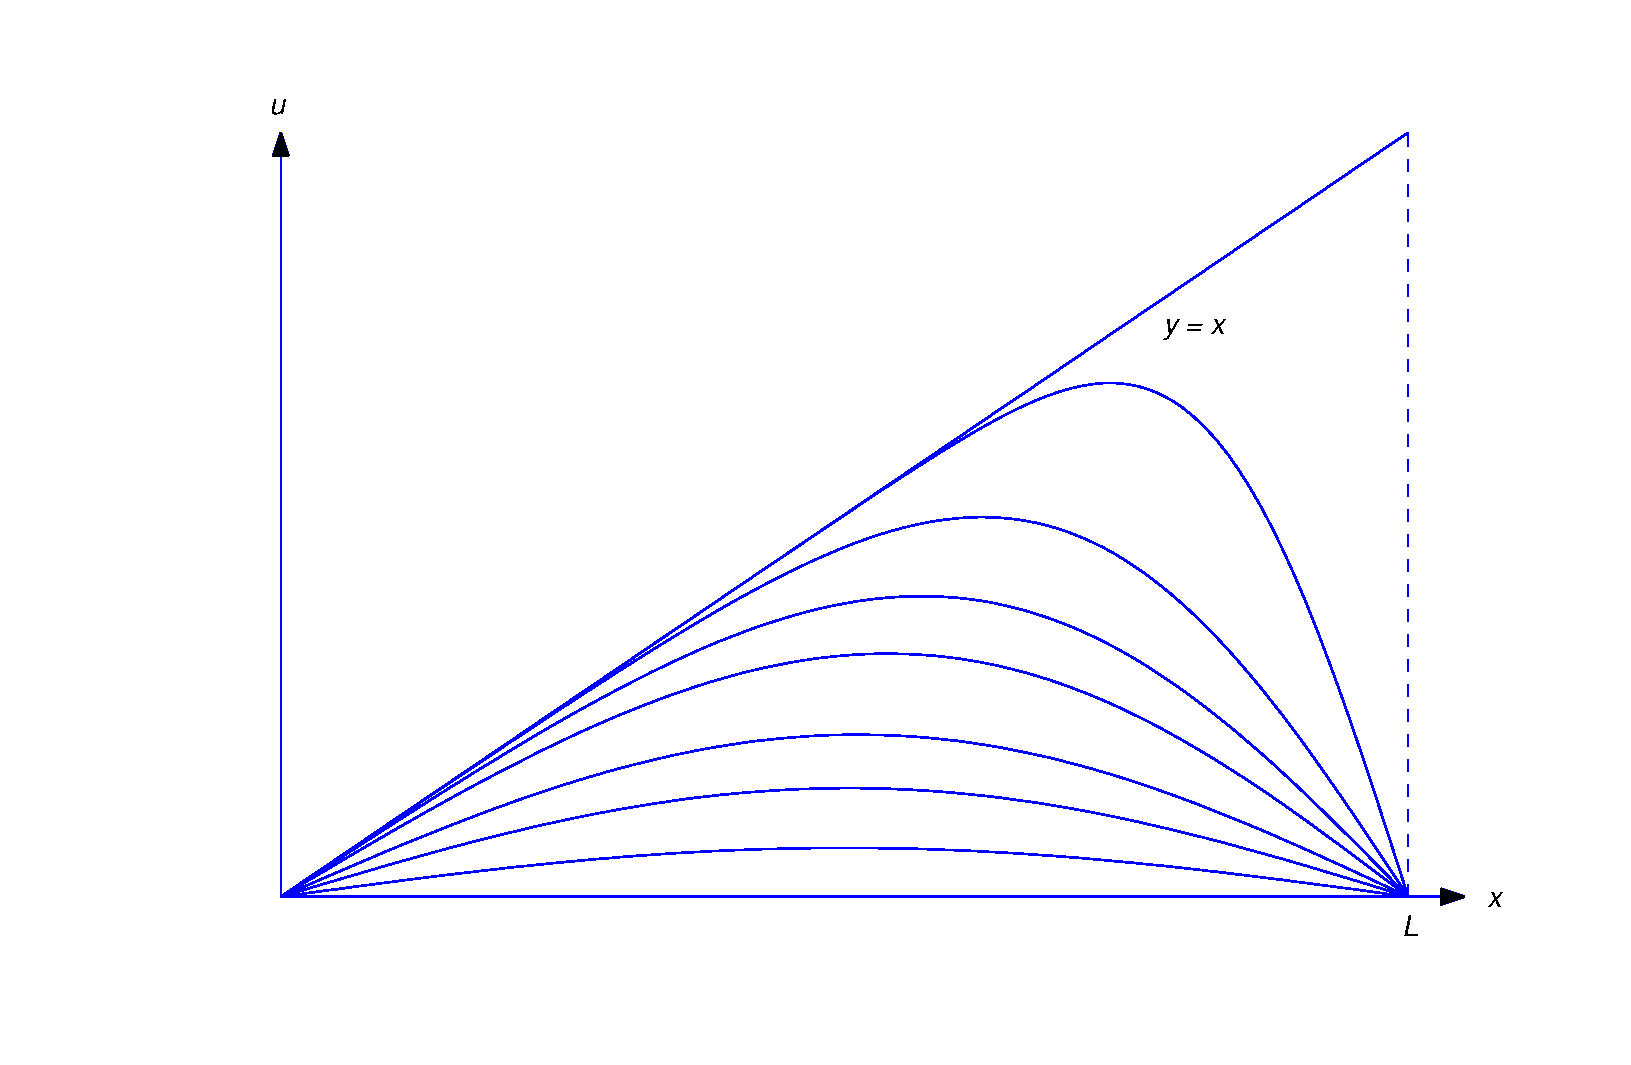
\includegraphics[bb=-78 148 689 643, width=5.67in, height=3.66in, keepaspectratio]{fig120102}
  \caption{}
  \label{figure:12.1.2}
\end{figure}

We leave it to you (Exercise~\ref{exer:12.1.3}) to use the method of separation of variables and
Theorem~\ref{thmtype:11.1.5} to motivate the next definition.

\begin{definition}
  \color{blue}
  \label{thmtype:12.1.5} \rm The formal solution of the initial-boundary value problem
  \begin{equation}
    \label{eq:12.1.8}
    \begin{array}{c}
      u_{t}=a^{2}u_{xx},\quad0<x<L,\quad t>0, \\
      u_{x}(0,t)=0,\quad u(L,t)=0,\quad t>0,  \\
      u(x,0)=f(x),\quad0\le x\le L
    \end{array}
  \end{equation}
  is
  \[
    u(x,t)=\sum_{n=1}^{\infty}\alpha_{n}e^{-(2n-1)^{2}\pi^{2}a^{2}t/4L^{2}}\cos\frac{(2n-1)\pi x}{2L},
  \]
  where
  \[
    C_{M}(x)=\sum_{n=1}^{\infty}\alpha_{n}\cos\frac{(2n-1)\pi x}{2L}
  \]
  is the mixed Fourier cosine series of $f$ on $[0,L]$; that is,
  \[
    \alpha_{n}=\frac{2}{L}\int_{0}^{L}f(x)\cos\frac{(2n-1)\pi x}{2L}\,dx.
  \]
\end{definition}

\begin{example}
  \label{example:12.1.4} \rm Solve \eqref{eq:12.1.8} with $f(x)=x-L$.
\end{example}

\solution From Example~\ref{example:11.3.3}, the mixed Fourier cosine series of $f$ on $[0,L]$ is
\[
  C_{M}(x)=-\frac{8L}{\pi^{2}}\sum_{n=1}^{\infty}\frac{1}{(2n-1)^{2}}\cos\frac{(2n-1)\pi x}{2L}.
\]
Therefore
\[
  u(x,t)=-\frac{8L}{\pi^{2}}\sum_{n=1}^{\infty}\frac{1}{(2n-1)^{2}}e^{-(2n-1)^{2}\pi^{2}a^{2}t/4L^{2}}\cos\frac{(2n-1)\pi x}{2L}.
\]

\boxit{Nonhomogeneous Problems}

\noindent
A problem of the form
\begin{equation}
  \label{eq:12.1.9}
  \begin{array}{c}
    u_{t}=a^{2}u_{xx}+h(x),\quad0<x<L,\quad t>0, \\
    u(0,t)=u_{0},\quad u(L,t)=u_{L},\quad t>0,   \\
    u(x,0)=f(x),\quad0\le x\le L
  \end{array}
\end{equation}
can be transformed to a problem that can be solved by separation of variables. We write
\begin{equation}
  \label{eq:12.1.10}u(x,t)=v(x,t)+q(x),
\end{equation}
where $q$ is to be determined. Then
\[
  u_{t}=v_{t}\mbox{\quad and \quad}u_{xx}=v_{xx}+q''
\]
so $u$ satisfies \eqref{eq:12.1.9} if $v$ satisfies
\[
  \begin{array}{c}
    v_{t}=a^{2}v_{xx}+a^{2}q''(x)+h(x),\quad0<x<L,\quad t>0, \\
    v(0,t)=u_{0}-q(0),\quad v(L,t)=u_{L}-q(L),\quad t>0,     \\
    v(x,0)=f(x)-q(x),\quad0\le x\le L.
  \end{array}
\]
This reduces to
\begin{equation}
  \label{eq:12.1.11}
  \begin{array}{c}
    v_{t}=a^{2}v_{xx},\quad0<x<L,\quad t>0, \\
    v(0,t)=0,\quad v(L,t)=0,\quad t>0,      \\
    v(x,0)=f(x)-q(x),\quad0\le x\le L
  \end{array}
\end{equation}
if
\[
  a^{2}q''+h(x)=0,\quad q(0)=u_{0},\quad q(L)=u_{L}.
\]
We can obtain $q$ by integrating $q''=-h/a^{2}$ twice and choosing the constants of integration so
that $q(0)=u_{0}$ and $q(L)=u_{L}$. Then we can solve \eqref{eq:12.1.11} for $v$ by separation of
variables, and \eqref{eq:12.1.10} is the solution of \eqref{eq:12.1.9}.

\begin{example}
  \label{example:12.1.5} \rm Solve
  \[
    \begin{array}{c}
      u_{t}=u_{xx}-2,\quad0<x<1,\quad t>0,      \\
      u(0,t)=-1,\quad u(1,t)=1,\quad t>0,       \\
      u(x,0)=x^{3}-2x^{2}+3x-1,\quad0\le x\le1.
    \end{array}
  \]

  \solution We leave it to you to show that
  \[
    q(x)=x^{2}+x-1
  \]
  satisfies
  \[
    q''-2=0,\quad q(0)=-1,\quad q(1)=1.
  \]
  Therefore
  \[
    u(x,t)=v(x,t)+x^{2}+x-1,
  \]
  where
  \[
    v_{t}=v_{xx},\quad0<x<1,\quad t>0,
  \]
  \[
    v(0,t)=0,\quad v(1,t)=0,\quad t>0,
  \]
  and
  \[
    v(x,0)=x^{3}-2x^{2}+3x-1-x^{2}-x+1=x(x^{2}-3x+2).
  \]
  From Example~\ref{example:12.1.1} with $a=1$ and $L=1$,
  \[
    v(x,t)= \frac{12}{\pi^{3}}\sum_{n=1}^{\infty}\frac{1}{n^{3}}e^{-n^{2}\pi^{2}t}\sin n\pi x.
  \]
  Therefore
  \[
    u(x,t)=x^{2}+x-1+ \frac{12}{\pi^{3}}\sum_{n=1}^{\infty}\frac{1}{n^{3}}e^{-n^{2}\pi^{2}t}\sin n\pi x. \eqno{\bbox}
  \]
\end{example}

A similar procedure works if the boundary conditions in \eqref{eq:12.1.11} are replaced by mixed
boundary conditions
\[
  u_{x}(0,t)=u_{0},\quad u(L,t)=u_{L},\quad t>0
\]
or
\[
  u(0,t)=u_{0},\quad u_{x}(L,t)=u_{L},\quad t>0;
\]
however, this isn't true in general for the boundary conditions
\[
  u_{x}(0,t)=u_{0},\quad u_{x}(L,t)=u_{L},\quad t>0.
\]
(See Exercise~\ref{exer:12.1.47}.)

\technology
\medskip
Numerical experiments can enhance your understanding of the solutions of initial-boundary value
problems. To be specific, consider the formal solution
\[
  u(x,t)=\sum_{n=1}^{\infty}\alpha_{n}e^{-n^{2}\pi^{2}a^{2}t/L^{2}}\sin\frac{n\pi x}{L},
\]
of \eqref{eq:12.1.4}, where
\[
  S(x)=\sum_{n=1}^{\infty}\alpha_{n}\sin\frac{n\pi x}{L}
\]
is the Fourier sine series of $f$ on $[0,L]$. Consider the $m$-th partial sum
\begin{equation}
  \label{eq:12.1.12}u_{m}(x,t)=\sum_{n=1}^{m}\alpha_{n}e^{-n^{2}\pi^{2}a^{2}t/L^{2}}\sin\frac{n\pi x}{L}.
\end{equation}
For several fixed values of $t$ (including $t=0$), graph $u_{m}(x,t)$ versus $t$. In some cases it
may be useful to graph the curves corresponding to the various values of $t$ on the same axes in
other cases you may want to graph the various curves successively (for increasing values of $t$),
and create a primitive motion picture on your monitor. Repeat this experiment for several values of
$m$, to compare how the results depend upon $m$ for small and large values of $t$. However, keep in
mind that the meanings of ``small'' and ``large'' in this case depend upon the constants $a^{2}$ and
$L^{2}$. A good way to handle this is to rewrite \eqref{eq:12.1.12} as
\[
  u_{m}(x,t)=\sum_{n=1}^{m}\alpha_{n}e^{-n^{2}\tau}\sin\frac{n\pi x}{L},
\]
where
\begin{equation}
  \label{eq:12.1.13}\tau=\frac{\pi^{2}a^{2}t}{L^{2}},
\end{equation}
and graph $u_{m}$ versus $x$ for selected values of $\tau$.

These comments also apply to the situations considered in
Definitions~\ref{thmtype:12.1.3}-\ref{thmtype:12.1.5}, except that \eqref{eq:12.1.13} should be
replaced by
\[
  \tau=\frac{\pi^{2}a^{2}t}{4L^{2}},
\]
in Definitions~\ref{thmtype:12.1.4} and \ref{thmtype:12.1.5}.

In some of the exercises we say ``perform numerical experiments.'' This means that you should
perform the computations just described with the formal solution obtained in the exercise.

\newpage

\exercises
\begin{exerciselist}
  \item\label{exer:12.1.1} Explain Definition~\ref{thmtype:12.1.3}.

  \item\label{exer:12.1.2} Explain Definition~\ref{thmtype:12.1.4}.

  \item\label{exer:12.1.3} Explain Definition~\ref{thmtype:12.1.5}.

  \item\label{exer:12.1.4} \Cex Perform numerical experiments with the formal solution obtained in
        Example~\ref{example:12.1.1}.

  \item\label{exer:12.1.5} \Cex Perform numerical experiments with the formal solution obtained in
        Example~\ref{example:12.1.2}.

  \item\label{exer:12.1.6} \Cex Perform numerical experiments with the formal solution obtained in
        Example~\ref{example:12.1.3}.

  \item\label{exer:12.1.7} \Cex Perform numerical experiments with the formal solution obtained in
        Example~\ref{example:12.1.4}.

  \exercisetext{In Exercises~\ref{exer:12.1.8}-\ref{exer:12.1.42} solve the initial-boundary value
  problem. Where indicated by \Cex, perform numerical experiments. To simplify the computation of
  coefficients in some of these problems, check first to see if $u(x,0)$ is a polynomial that
  satisfies the boundary conditions. If it does, apply Theorem~\ref{thmtype:11.3.5}; also, see
  Exercises~$11.3$.~\hspace*{-3pt}\ref{exer:11.3.35}\part{b},
  $11.3$.~\hspace*{-3pt}\ref{exer:11.3.42}\part{b}, and
  $11.3$.~\hspace*{-3pt}\ref{exer:11.3.50}\part{b}.}

  \item\label{exer:12.1.8} $u_{t}=u_{xx},\quad0<x<1,\quad t>0$,\\ $u(0,t)=0,\quad u(1,t)=0,\quad t>0$,\\ $u(x,0)=x(1-x),\quad0\le x\le1$

  \item\label{exer:12.1.9} $u_{t}=9u_{xx},\quad0<x<4,\quad t>0$,\\ $u(0,t)=0,\quad u(4,t)=0,\quad t>0$,\\ $u(x,0)=1,\quad0\le x\le4$

  \item\label{exer:12.1.10} $u_{t}=3u_{xx},\quad0<x<\pi,\quad t>0$,\\ $u(0,t)=0,\quad u(\pi,t)=0,\quad t>0$,\\ $u(x,0)=x\sin x,\quad0\le x\le\pi$

  \item\label{exer:12.1.11} \Cex $u_{t}=9u_{xx},\quad0<x<2,\quad t>0$,\\ $u(0,t)=0,\quad u(2,t)=0,\quad t>0$,\\ $u(x,0)=x^{2}(2-x),\quad0\le x\le2$

  \item\label{exer:12.1.12} $u_{t}=4u_{xx},\quad0<x<3,\quad t>0$,\\ $u(0,t)=0,\quad u(3,t)=0,\quad t>0$,\\ $u(x,0)=x(9-x^{2}),\quad0\le x\le3$

  \item\label{exer:12.1.13} $u_{t}=4u_{xx},\quad0<x<2,\quad t>0$,\\ $u(0,t)=0,\quad u(2,t)=0,\quad t>0$,\\ $u(x,0)= \left\{
  \begin{array}{cl}
    x,   & 0\le x\le1, \\
    2-x, & 1\le x\le2.
  \end{array}\right.$

  \item\label{exer:12.1.14} $u_{t}=7u_{xx},\quad0<x<1,\quad t>0$,\\ $u(0,t)=0,\quad u(1,t)=0,\quad t>0$,\\ $u(x,0)=x(3x^{4}-10x^{2}+7),\quad0\le x\le1$

  \item\label{exer:12.1.15} $u_{t}=5u_{xx},\quad0<x<1,\quad t>0$,\\ $u(0,t)=0,\quad u(1,t)=0,\quad t>0$,\\ $u(x,0)=x(x^{3}-2x^{2}+1),\quad0\le x\le1$

  \item\label{exer:12.1.16} $u_{t}=2u_{xx},\quad0<x<1,\quad t>0$,\\ $u(0,t)=0,\quad u(1,t)=0,\quad t>0$,\\ $u(x,0)=x(3x^{4}-5x^{3}+2),\quad0\le x\le1$

  \item\label{exer:12.1.17} \Cex $u_{t}=9u_{xx},\quad0<x<4,\quad t>0$,\\ $u_{x}(0,t)=0,\quad u_{x}(4,t)=0,\quad t>0$,\\ $u(x,0)=x^{2},\quad0\le x\le4$

  \item\label{exer:12.1.18} $u_{t}=4u_{xx},\quad0<x<2,\quad t>0$,\\ $u_{x}(0,t)=0,\quad u_{x}(2,t)=0,\quad t>0$,\\ $u(x,0)=x(x-4),\quad0\le x\le2$

  \item\label{exer:12.1.19} \Cex $u_{t}=9u_{xx},\quad0<x<1,\quad t>0$,\\ $u_{x}(0,t)=0,\quad u_{x}(1,t)=0,\quad t>0$,\\ $u(x,0)=x(1-x),\quad0\le x\le1$

  \item\label{exer:12.1.20} $u_{t}=3u_{xx},\quad0<x<2,\quad t>0$,\\ $u_{x}(0,t)=0,\quad u_{x}(2,t)=0,\quad t>0$,\\ $u(x,0)=2x^{2}(3-x),\quad0\le x\le2$

  \item\label{exer:12.1.21} $u_{t}=5u_{xx},\quad0<x<\sqrt{2},\quad t>0$,\\ $u_{x}(0,t)=0,\quad u_{x}(\sqrt{2},t)=0,\quad t>0$,\\ $u(x,0)=3x^{2}(x^{2}-4),\quad0\le x\le\sqrt{2}$

  \item\label{exer:12.1.22} \Cex $u_{t}=3u_{xx},\quad0<x<1,\quad t>0$,\\ $u_{x}(0,t)=0,\quad u_{x}(1,t)=0,\quad t>0$,\\ $u(x,0)=x^{3}(3x-4),\quad0\le x\le1$

  \item\label{exer:12.1.23} $u_{t}=u_{xx},\quad0<x<1,\quad t>0$,\\ $u_{x}(0,t)=0,\quad u_{x}(1,t)=0,\quad t>0$,\\ $u(x,0)=x^{2}(3x^{2}-8x+6),\quad0\le x\le1$

  \item\label{exer:12.1.24} $u_{t}=u_{xx},\quad0<x<\pi,\quad t>0$,\\ $u_{x}(0,t)=0,\quad u_{x}(\pi,t)=0,\quad t>0$,\\ $u(x,0)=x^{2}(x-\pi)^{2},\quad0\le x\le\pi$

  \item\label{exer:12.1.25} $u_{t}=u_{xx},\quad0<x<1,\quad t>0$,\\ $u(0,t)=0,\quad u_{x}(1,t)=0,\quad t>0$,\\ $u(x,0)=\sin\pi x,\quad0\le x\le1$

  \item\label{exer:12.1.26} \Cex $u_{t}=3u_{xx},\quad0<x<\pi,\quad t>0$,\\ $u(0,t)=0,\quad u_{x}(\pi,t)=0,\quad t>0$,\\ $u(x,0)=x(\pi-x),\quad0\le x\le\pi$

  \item\label{exer:12.1.27} $u_{t}=5u_{xx},\quad0<x<2,\quad t>0$,\\ $u(0,t)=0,\quad u_{x}(2,t)=0,\quad t>0$,\\ $u(x,0)=x(4-x),\quad0\le x\le2$

  \item\label{exer:12.1.28} $u_{t}=u_{xx},\quad0<x<1,\quad t>0$,\\ $u(0,t)=0,\quad u_{x}(1,t)=0,\quad t>0$,\\ $u(x,0)=x^{2}(3-2x),\quad0\le x\le1$

  \item\label{exer:12.1.29} $u_{t}=u_{xx},\quad0<x<1,\quad t>0$,\\ $u(0,t)=0,\quad u_{x}(1,t)=0,\quad t>0$,\\ $u(x,0)=(x-1)^{3}+1,\quad0\le x\le1$

  \item\label{exer:12.1.30} \Cex $u_{t}=u_{xx},\quad0<x<1,\quad t>0$,\\ $u(0,t)=0,\quad u_{x}(1,t)=0,\quad t>0$,\\ $u(x,0)=x(x^{2}-3),\quad0\le x\le1$

  \item\label{exer:12.1.31} $u_{t}=u_{xx},\quad0<x<1,\quad t>0$,\\ $u(0,t)=0,\quad u_{x}(1,t)=0,\quad t>0$,\\ $u(x,0)=x^{3}(3x-4),\quad0\le x\le1$

  \item\label{exer:12.1.32} $u_{t}=u_{xx},\quad0<x<1,\quad t>0$,\\ $u(0,t)=0,\quad u_{x}(1,t)=0,\quad t>0$,\\ $u(x,0)=x(x^{3}-2x^{2}+2),\quad0\le x\le1$

  \item\label{exer:12.1.33} $u_{t}=3u_{xx},\quad0<x<\pi,\quad t>0$,\\ $u_{x}(0,t)=0,\quad u(\pi,t)=0,\quad t>0$,\\ $u(x,0)=x^{2}(\pi-x),\quad0\le x\le\pi$

  \item\label{exer:12.1.34} $u_{t}=16u_{xx},\quad0<x<2\pi,\quad t>0$,\\ $u_{x}(0,t)=0,\quad u(2\pi,t)=0,\quad t>0$,\\ $u(x,0)=4,\quad0\le x\le2\pi$

  \item\label{exer:12.1.35} $u_{t}=9u_{xx},\quad0<x<4,\quad t>0$,\\ $u_{x}(0,t)=0,\quad u(4,t)=0,\quad t>0$,\\ $u(x,0)=x^{2},\quad0\le x\le4$

  \item\label{exer:12.1.36} \Cex $u_{t}=3u_{xx},\quad0<x<1,\quad t>0$,\\ $u_{x}(0,t)=0,\quad u(1,t)=0,\quad t>0$,\\ $u(x,0)=1-x,\quad0\le x\le1$

  \item\label{exer:12.1.37} $u_{t}=u_{xx},\quad0<x<1,\quad t>0$,\\ $u_{x}(0,t)=0,\quad u(1,t)=0,\quad t>0$,\\ $u(x,0)=1-x^{3},\quad0\le x\le1$

  \item\label{exer:12.1.38} $u_{t}=7u_{xx},\quad0<x<\pi,\quad t>0$,\\ $u_{x}(0,t)=0,\quad u(\pi,t)=0,\quad t>0$,\\ $u(x,0)=\pi^{2}-x^{2},\quad0\le x\le\pi$

  \item\label{exer:12.1.39} $u_{t}=u_{xx},\quad0<x<1,\quad t>0$,\\ $u_{x}(0,t)=0,\quad u(1,t)=0,\quad t>0$,\\ $u(x,0)=4x^{3}+3x^{2}-7,\quad0\le x\le1$

  \item\label{exer:12.1.40} $u_{t}=u_{xx},\quad0<x<1,\quad t>0$,\\ $u_{x}(0,t)=0,\quad u(1,t)=0,\quad t>0$,\\ $u(x,0)=2x^{3}+3x^{2}-5,\quad0\le x\le1$

  \item\label{exer:12.1.41} \Cex $u_{t}=u_{xx},\quad0<x<1,\quad t>0$,\\ $u_{x}(0,t)=0,\quad u(1,t)=0,\quad t>0$,\\ $u(x,0)=x^{4}-4x^{3}+6x^{2}-3,\quad0\le x\le1$

  \item\label{exer:12.1.42} $u_{t}=u_{xx},\quad0<x<1,\quad t>0$,\\ $u_{x}(0,t)=0,\quad u(1,t)=0,\quad t>0$,\\ $u(x,0)=x^{4}-2x^{3}+1,\quad0\le x\le1$

  \exercisetext{In Exercises~\ref{exer:12.1.43}-\ref{exer:12.1.46} solve the initial-boundary value
  problem. Perform numerical experiments for specific values of $L$ and $a$.}

  \item\label{exer:12.1.43} \Cex $u_{t}=a^{2}u_{xx},\quad0<x<L,\quad t>0$,\\ $u_{x}(0,t)=0,\quad u_{x}(L,t)=0,\quad t>0$,\\ $u(x,0)= \left\{
  \begin{array}{cl}
    1, & 0\le x\le\frac{L}{2}, \\
    0, & \frac{L}{2}<x<L
  \end{array}\right.$

  \item\label{exer:12.1.44} \Cex $u_{t}=a^{2}u_{xx},\quad0<x<L,\quad t>0$,\\ $u(0,t)=0,\quad u(L,t)=0,\quad t>0$,\\ $u(x,0)= \left\{
  \begin{array}{cl}
    1, & 0\le x\le\frac{L}{2}, \\
    0, & \frac{L}{2}<x<L
  \end{array}\right.$

  \item\label{exer:12.1.45} \Cex $u_{t}=a^{2}u_{xx},\quad0<x<L,\quad t>0$,\\ $u_{x}(0,t)=0,\quad u(L,t)=0,\quad t>0$,\\ $u(x,0)= \left\{
  \begin{array}{cl}
    1, & 0\le x\le\frac{L}{2}, \\
    0, & \frac{L}{2}<x<L
  \end{array}\right.$

  \item\label{exer:12.1.46} \Cex $u_{t}=a^{2}u_{xx},\quad0<x<L,\quad t>0$,\\ $u(0,t)=0,\quad u_{x}(L,t)=0,\quad t>0$,\\ $u(x,0)= \left\{
  \begin{array}{cl}
    1, & 0\le x\le\frac{L}{2}, \\
    0, & \frac{L}{2}<x<L
  \end{array}\right.$

  \item\label{exer:12.1.47} Let $h$ be continuous on $[0,L]$ and let $u_{0}$, $u_{L}$, and $a$ be
        constants, with $a>0$. Show that it's always possible to find a function $q$ that satisfies
        \part{a}, \part{b}, or \part{c}, but that this isn't so for \part{d}.
  \begin{alist}
    \item % (a)
    $a^{2}q''+h=0,\quad q(0)=u_{0},\quad q(L)=u_{L}$

    \item % (b)
    $a^{2}q''+h=0,\quad q'(0)=u_{0},\quad q(L)=u_{L}$

    \item % (c)
    $a^{2}q''+h=0,\quad q(0)=u_{0},\quad q'(L)=u_{L}$

    \item % (d)
    $a^{2}q''+h=0,\quad q'(0)=u_{0},\quad q'(L)=u_{L}$
  \end{alist}

  \exercisetext{In Exercises~\ref{exer:12.1.48}-\ref{exer:12.1.53} solve the nonhomogeneous
  initial-boundary value problem}

  \item\label{exer:12.1.48} $u_{t}=9u_{xx}-54x,\quad0<x<4,\quad t>0$,\\ $u(0,t)=1,\quad u(4,t)=61,\quad t>0$,\\ $u(x,0)=2-x+x^{3},\quad0\le x\le4$

  \item\label{exer:12.1.49} $u_{t}=u_{xx}-2,\quad0<x<1,\quad t>0$,\\ $u(0,t)=1,\quad u(1,t)=3,\quad t>0$,\\ $u(x,0)=2x^{2}+1,\quad0\le x\le1$

  \item\label{exer:12.1.50} $u_{t}=3u_{xx}-18x,\quad0<x<1,\quad t>0$,\\ $u_{x}(0,t)=-1,\quad u(1,t)=-1,\quad t>0$,\\ $u(x,0)=x^{3}-2x,\quad0\le x\le1$

  \item\label{exer:12.1.51} $u_{t}=9u_{xx}-18,\quad0<x<4,\quad t>0$,\\ $u_{x}(0,t)=-1,\quad u(4,t)=10,\quad t>0$,\\ $u(x,0)=2x^{2}-x-2,\quad0\le x\le4$

  \item\label{exer:12.1.52} $u_{t}=u_{xx}+\pi^{2}\sin\pi x,\quad0<x<1,\quad t>0$,\\ $u(0,t)=0,\quad u_{x}(1,t)=-\pi,\quad t>0$,\\ $u(x,0)=2\sin\pi x,\quad0\le x\le1$

  \item\label{exer:12.1.53} $u_{t}=u_{xx}-6x,\quad0<x<L,\quad t>0$,\\ $u(0,t)=3,\quad u_{x}(1,t)=2,\quad t>0$,\\ $u(x,0)=x^{3}-x^{2}+x+3,\quad0\le x\le1$

  \item\label{exer:12.1.54} In this exercise take it as given that the infinite series
        $\sum_{n=1}^{\infty}n^{p}e^{-qn^{2}}$ converges for all $p$ if $q>0$, and, where
        appropriate, use the comparison test for absolute convergence of an infinite series.

  Let
  \[
    u(x,t)=\sum_{n=1}^{\infty}\alpha_{n}e^{-n^{2}\pi^{2} a^{2}t/L^{2}}\sin\frac{n\pi x}{L}
  \]
  where
  \[
    \alpha_{n}=\frac{2}{L}\int_{0}^{L}f(x)\sin\frac{n\pi x}{L}\,dx
  \]
  and $f$ is piecewise smooth on $[0,L]$.

  \begin{alist}
    \item % (a)
    Show that $u$ is defined for $(x,t)$ such that $t>0$.

    \item % (b)
    For fixed $t>0$, use Theorem~\ref{thmtype:12.1.2} with $z=x$ to show that
    \[
      u_{x}(x,t)=\frac{\pi}{L}\sum_{n=1}^{\infty}n\alpha_{n}e^{-n^{2}\pi^{2} a^{2}t/L^{2}}\cos\frac{n\pi x}{L},\quad-\infty<x<\infty.
    \]

    \item % (c)
    Starting from the result of \part{a}, use Theorem~\ref{thmtype:12.1.2} with $z=x$ to show that,
    for a fixed $t>0$,
    \[
      u_{xx}(x,t)=-\frac{\pi^{2}}{L^{2}}\sum_{n=1}^{\infty}n^{2}\alpha_{n}e^{-n^{2}\pi^{2}a^{2}t/L^{2}}\sin\frac{n\pi x}{L},\quad-\infty<x<\infty.
    \]

    \item % (d)
    For fixed but arbitrary $x$, use Theorem~\ref{thmtype:12.1.2} with $z=t$ to show that
    \[
      u_{t}(x,t)=-\frac{\pi^{2}a^{2}}{L^{2}}\sum_{n=1}^{\infty}n^{2}\alpha_{n}e^{-n^{2}\pi^{2}a^{2}t/L^{2}}\sin\frac{n\pi x}{L},
    \]
    if $t>t_{0}>0$, where $t_{0}$ is an arbitrary positive number. Then argue that since $t_{0}$ is
    arbitrary, the conclusion holds for all $t>0$.

    \item % (e)
    Conclude from \part{c} and \part{d} that
    \[
      u_{t}=a^{2}u_{xx},\quad-\infty<x<\infty,\quad t>0.
    \]
  \end{alist}

  By repeatedly applying the arguments in \part{a} and \part{c}, it can be shown that $u$ can be
  differentiated term by term any number of times with respect to $x$ and/or $t$ if $t>0$.
\end{exerciselist}
